% 第 16 题直三棱柱图：按固定源 PDF 内容流实测值换算（1 bp → 0.03515 cm）。
% 原点取顶点 A（源页 (668.81, 348.86) pdf 坐标），y 向上。
% 顶点全部为排版源值（LaTeX 矢量 PDF）：D 为 AB₁ 精确中点、E 为 B₁C∩BC₁（t=0.5），均已数值复核。
% 实线 11 段（前侧棱 B₁B 可见故实、下底后边 A₁C₁ 隐藏故虚）；虚线 2 段；图内无点标记。
% 虚线样式照源 [2.98883 2.98883]。
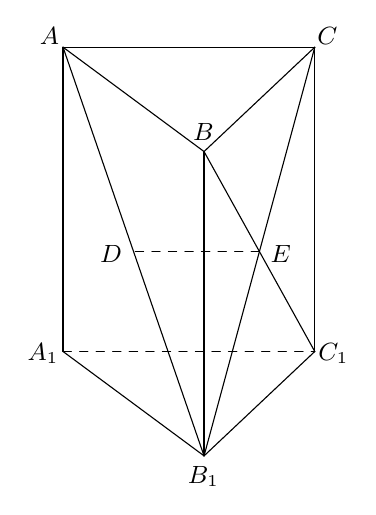
\begin{tikzpicture}[line cap=round,line join=round,font=\small,x=0.03515cm,y=0.03515cm]
% ===== 实线（11 段）=====
\draw (0,0)--(50.94,-147.63);  % A–B1 侧面 ABB₁A₁ 对角线，过 D
\draw (0,-109.93)--(50.94,-147.63);  % A1–B1 下底边
\draw (50.94,-147.63)--(90.94,-109.93);  % B1–C1 下底边
\draw (0,-109.93)--(0,0);  % A1–A 左侧棱（竖直）
\draw (50.94,-147.63)--(50.94,-37.7);  % B1–B 前侧棱（竖直，可见）
\draw (90.94,-109.93)--(90.94,0);  % C1–C 右侧棱（竖直）
\draw (0,0)--(50.94,-37.7);  % A–B 上底边
\draw (50.94,-37.7)--(90.94,0);  % B–C 上底边
\draw (90.94,0)--(0,0);  % C–A 上底边（水平）
\draw (50.94,-147.63)--(90.94,0);  % B1–C 侧面 BCC₁B₁ 对角线，过 E
\draw (90.94,-109.93)--(50.94,-37.7);  % C1–B 同侧面另一对角线，过 E
% ===== 虚线（2 段）=====
\draw[dash pattern=on 2.99pt off 2.99pt] (0,-109.93)--(90.94,-109.93);  % A1–C1 下底面后边（隐藏棱）
\draw[dash pattern=on 2.99pt off 2.99pt] (70.94,-73.81)--(25.47,-73.81);  % E–D D、E 连线（水平）
% ===== 标注（照源字框中心，显式坐标）=====
\node[anchor=center,inner sep=0] at (-4.93,3.975) {\(A\)};
\node[anchor=center,inner sep=0] at (95.495,3.975) {\(C\)};
\node[anchor=center,inner sep=0] at (50.675,-30.69) {\(B\)};
\node[anchor=center,inner sep=0] at (17.355,-74.775) {\(D\)};
\node[anchor=center,inner sep=0] at (78.605,-74.775) {\(E\)};
\node[anchor=center,inner sep=0] at (-7.225,-110.55) {\(A_{1}\)};
\node[anchor=center,inner sep=0] at (97.66,-110.55) {\(C_{1}\)};
\node[anchor=center,inner sep=0] at (50.685,-155.22) {\(B_{1}\)};
\end{tikzpicture}
